% In principle, this file can be redistributed and/or modified under
% the terms of the GNU Public License, version 2.


\documentclass{beamer}
\usepackage{adjustbox}
%\usetheme{AnnArbor}
%\usetheme{Antibes}
%\usetheme{Bergen}
%\usetheme{Berkeley}
%\usetheme{Berlin}
%\usetheme{Boadilla}
%\usetheme{boxes}
%\usetheme{CambridgeUS}
%\usetheme{Copenhagen}
%\usetheme{Darmstadt}
%\usetheme{default}
%\usetheme{Frankfurt}
%\usetheme{Goettingen}
%\usetheme{Hannover}
%\usetheme{Ilmenau}
%\usetheme{JuanLesPins}
%\usetheme{Luebeck}
\usetheme{Madrid}
%\usetheme{Malmoe}
%\usetheme{Marburg}
%\usetheme{Montpellier}
%\usetheme{PaloAlto}
%\usetheme{Pittsburgh}
%\usetheme{Rochester}
%\usetheme{Singapore}
%\usetheme{Szeged}
%\usetheme{Warsaw}
\usepackage[utf8]{inputenc}

\title{Prostate Adenocaricome Insights}

\subtitle{Gene Expression approach from TCGA RNA-seq data}

\author{A. Auladell\inst{1}, J. Martí \inst{1} \& D. Mas\inst{1}}

\institute[UPF] 
{
  \inst{1}%
  Department of Experimental \& Health Science\\
  Universitat Pompeu Fabra
}

\date{\today}

\subject{IEO: Information Extraction from Omics technologies}
% This is only inserted into the PDF information catalog. Can be left
% out. 

% If you have a file called "university-logo-filename.xxx", where xxx
% is a graphic format that can be processed by latex or pdflatex,
% resp., then you can add a logo as follows:

\pgfdeclareimage[height=1cm]{upf-logo}{upf.png}
\logo{\pgfuseimage{upf-logo}}

% Delete this, if you do not want the table of contents to pop up at
% the beginning of each subsection:
\AtBeginSection[]
{
  \begin{frame}<beamer>{Outline}
    \tableofcontents[currentsection]
  \end{frame}
}

% Let's get started
\begin{document}

\begin{frame}
  \titlepage
\end{frame}

\begin{frame}{Outline}
  \tableofcontents
  % You might wish to add the option [pausesections]
\end{frame}

% Section and subsections will appear in the presentation overview
% and table of contents.
\section{Introduction}

\subsection{Prostate cancer generalities}
\begin{frame}{Introduction}{Prostate cancer generalities}
  	\begin{block}{Incidence}
		\begin{itemize}
		\item 1 in 7 men will be diagnosed during his lifespan.
		\item 2nd deadliest cancer type in males.
		\item Higher prevalence in African Ancestry.
		\end{itemize}
	\end{block}
	\pause % The slide will pause after showing the first item
	\begin{block}{Previous studies}
		\begin{itemize}
		\item Other RNA-seq studies have been published, most of them at gene level.
		\item The TCGA Consortium gathered a big cohort of patients and have performed several tests and sequencing techniques.
		\end{itemize}
	\end{block}
\end{frame}

\subsection{The Genome Cancer Atlas article}

% You can reveal the parts of a slide one at a time
% with the \pause command:
\begin{frame}{Introduction}{TGCA \cite{Abeshouse2015}}
  \begin{itemize}
  \item<1-> {
    AIM: Create a molecular taxonomy of Prostate Cancer based on 333 tumor samples
    \pause % The slide will pause after showing the first item
  }
  \item<2-> {   
	Data: Whole-exome sequencing (somatic mutations); Array-based methods (somatic copy-number changes); DNA 		methylation and mRNA sequencing (Gene Expression)  
  }
  % You can also specify when the content should appear
  % by using <n->:
  \item<3-> {
    74\% of all tumors were identified in 7 different molecular subtypes: (1) ERG, (2) ETV1, (3) ETV4, or (4) FLI1, (5) SPOP, (6) FOXA1 or (7) IDH1.
  }
  \item<4-> {
  	No relationship between clinical data and molecular cancer subtype (p.e. Gleason score).
  }
  \item<5->{
  	However, subtypes did not share any particular expression pattern. 
  }
  \end{itemize}
\end{frame}

\section{Methods}

\subsection{Data Availability \& Experimental Design}

\begin{frame}{Methods}{Data Availability \& Experimental Design}
	\begin{block}{Data Availability}
		\begin{itemize}
			\item The original data was realised by Rahman et al. \cite{Rahman15112015} .
			\item Constructed with Rsubread/featureCounts \cite{Rsubread}.
			\item Curated by Robert Castelo-Valdueza.
			\item 52 normal samples vs. 502 tumor samples.
		\end{itemize}
	\end{block}
	
	\begin{block}{Experimental Design}
		\begin{itemize}
			\item Paired design with 50 normal samples vs. 50 tumor samples.
			\item After trimming, the design consisted of 42 normal samples vs. 42 tumor samples.
		\end{itemize}
	\end{block}

\end{frame}

\subsection{Processing}
\begin{frame}{Methods}{Processing}
	\begin{itemize}
		\item Normalization with DGE algorithm \cite{Robinson01012010} 20115 genes.
		\item Filtered transcripts with logCPM \textgreater 1, remaining 11722 genes.
		\item Batch effect evaluated by patient barcode  (which contains center, site and plate).
		\item Some samples where deprecated (1:1 ratio) as they disturbed the clustering of groups (mentioned before).
		\item Clustering algorithms and HeatMap visualisation were performed to assess possible biases.
	\end{itemize}

\end{frame}

\begin{frame}{Methods}{Data Display}
	\centering
	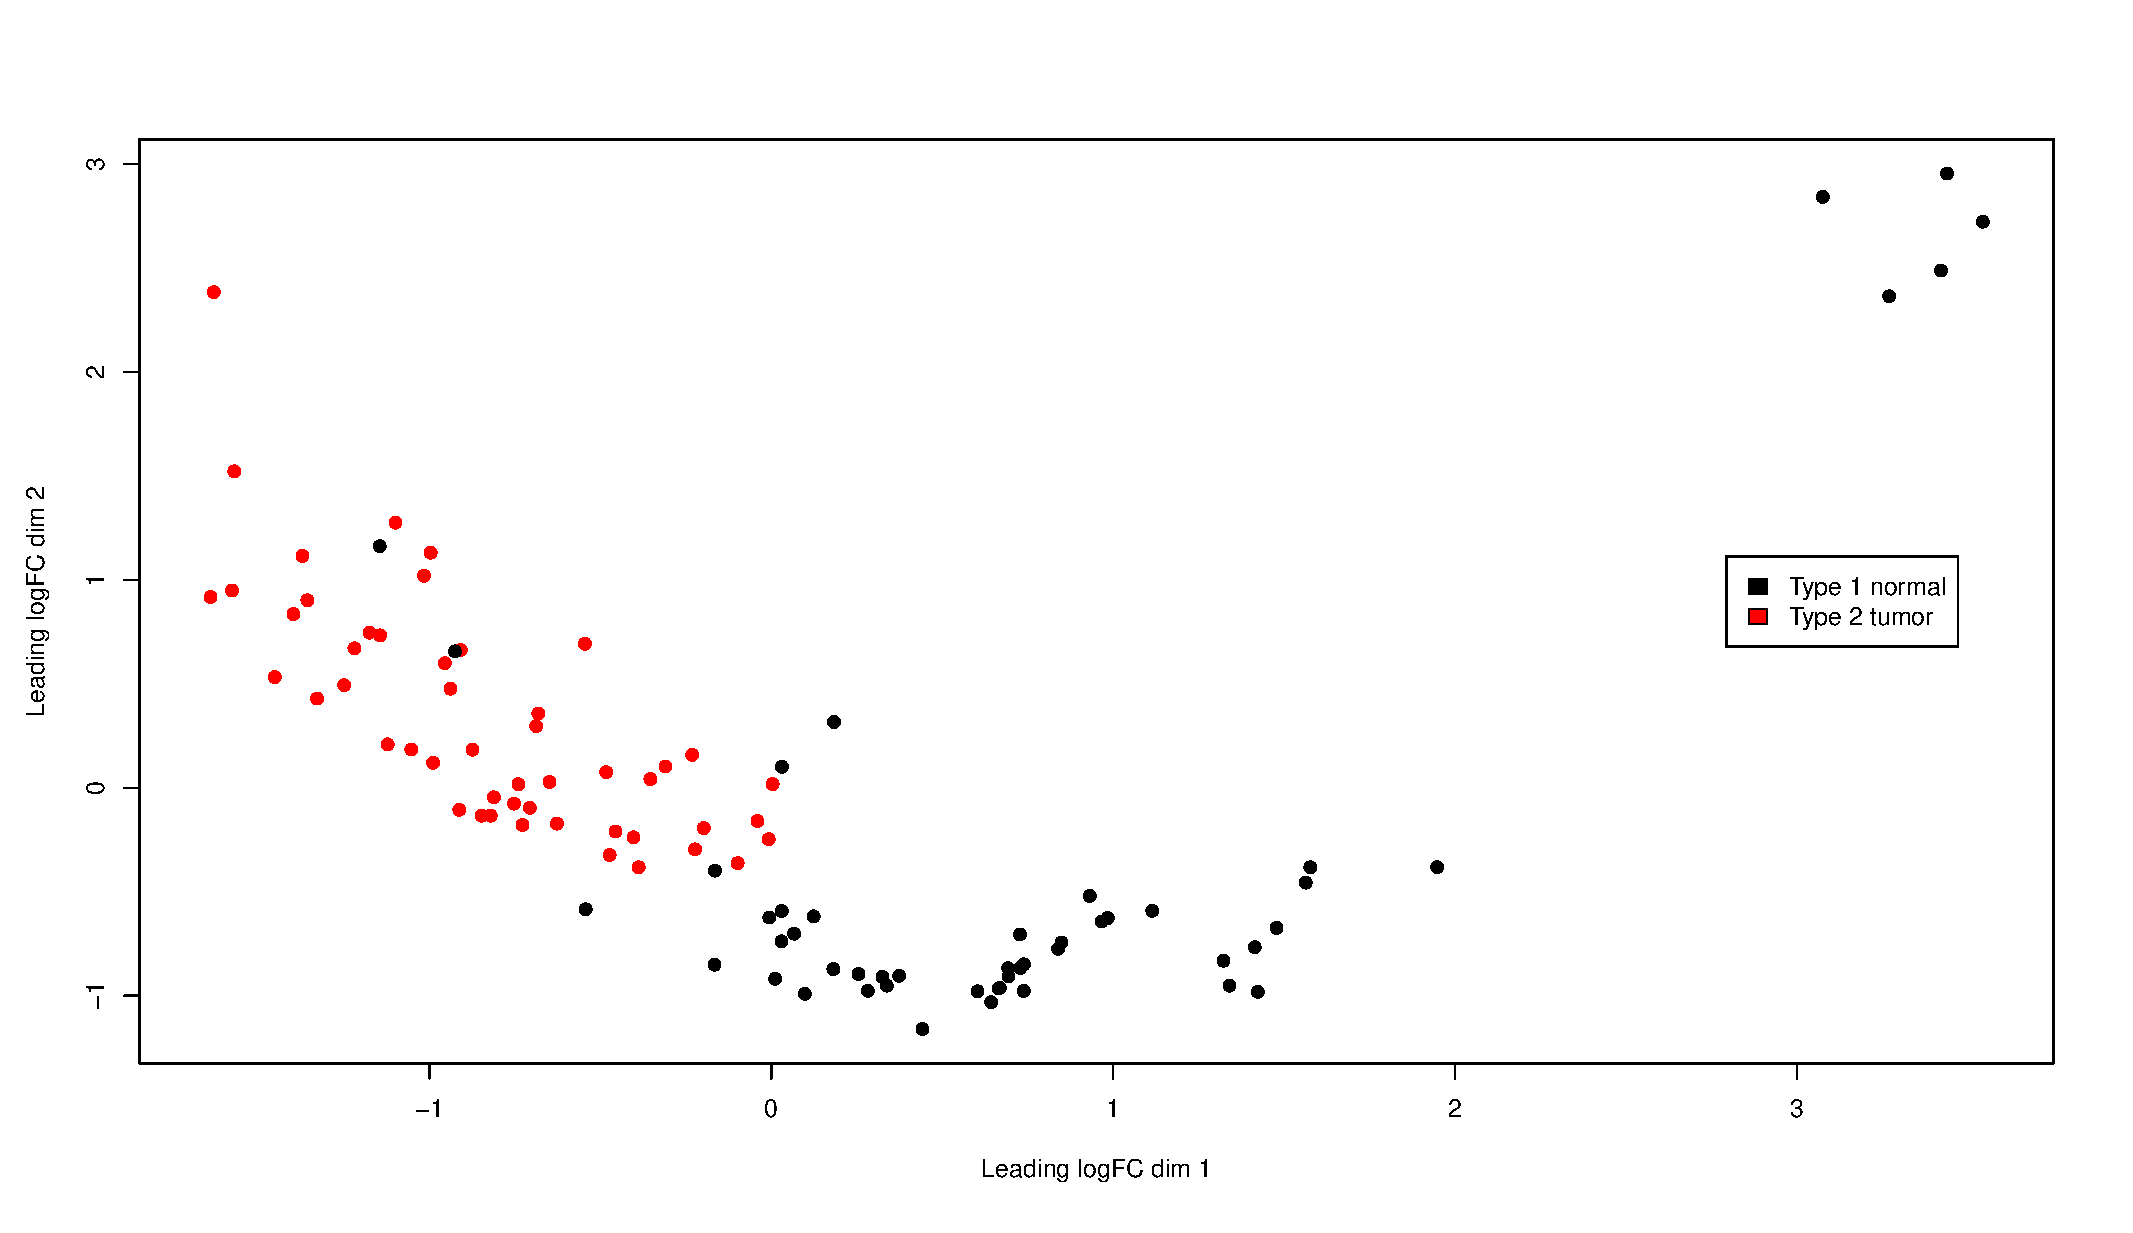
\includegraphics[width=0.8\textwidth,height=0.5\textheight,keepaspectratio]{mds2-1.eps}

	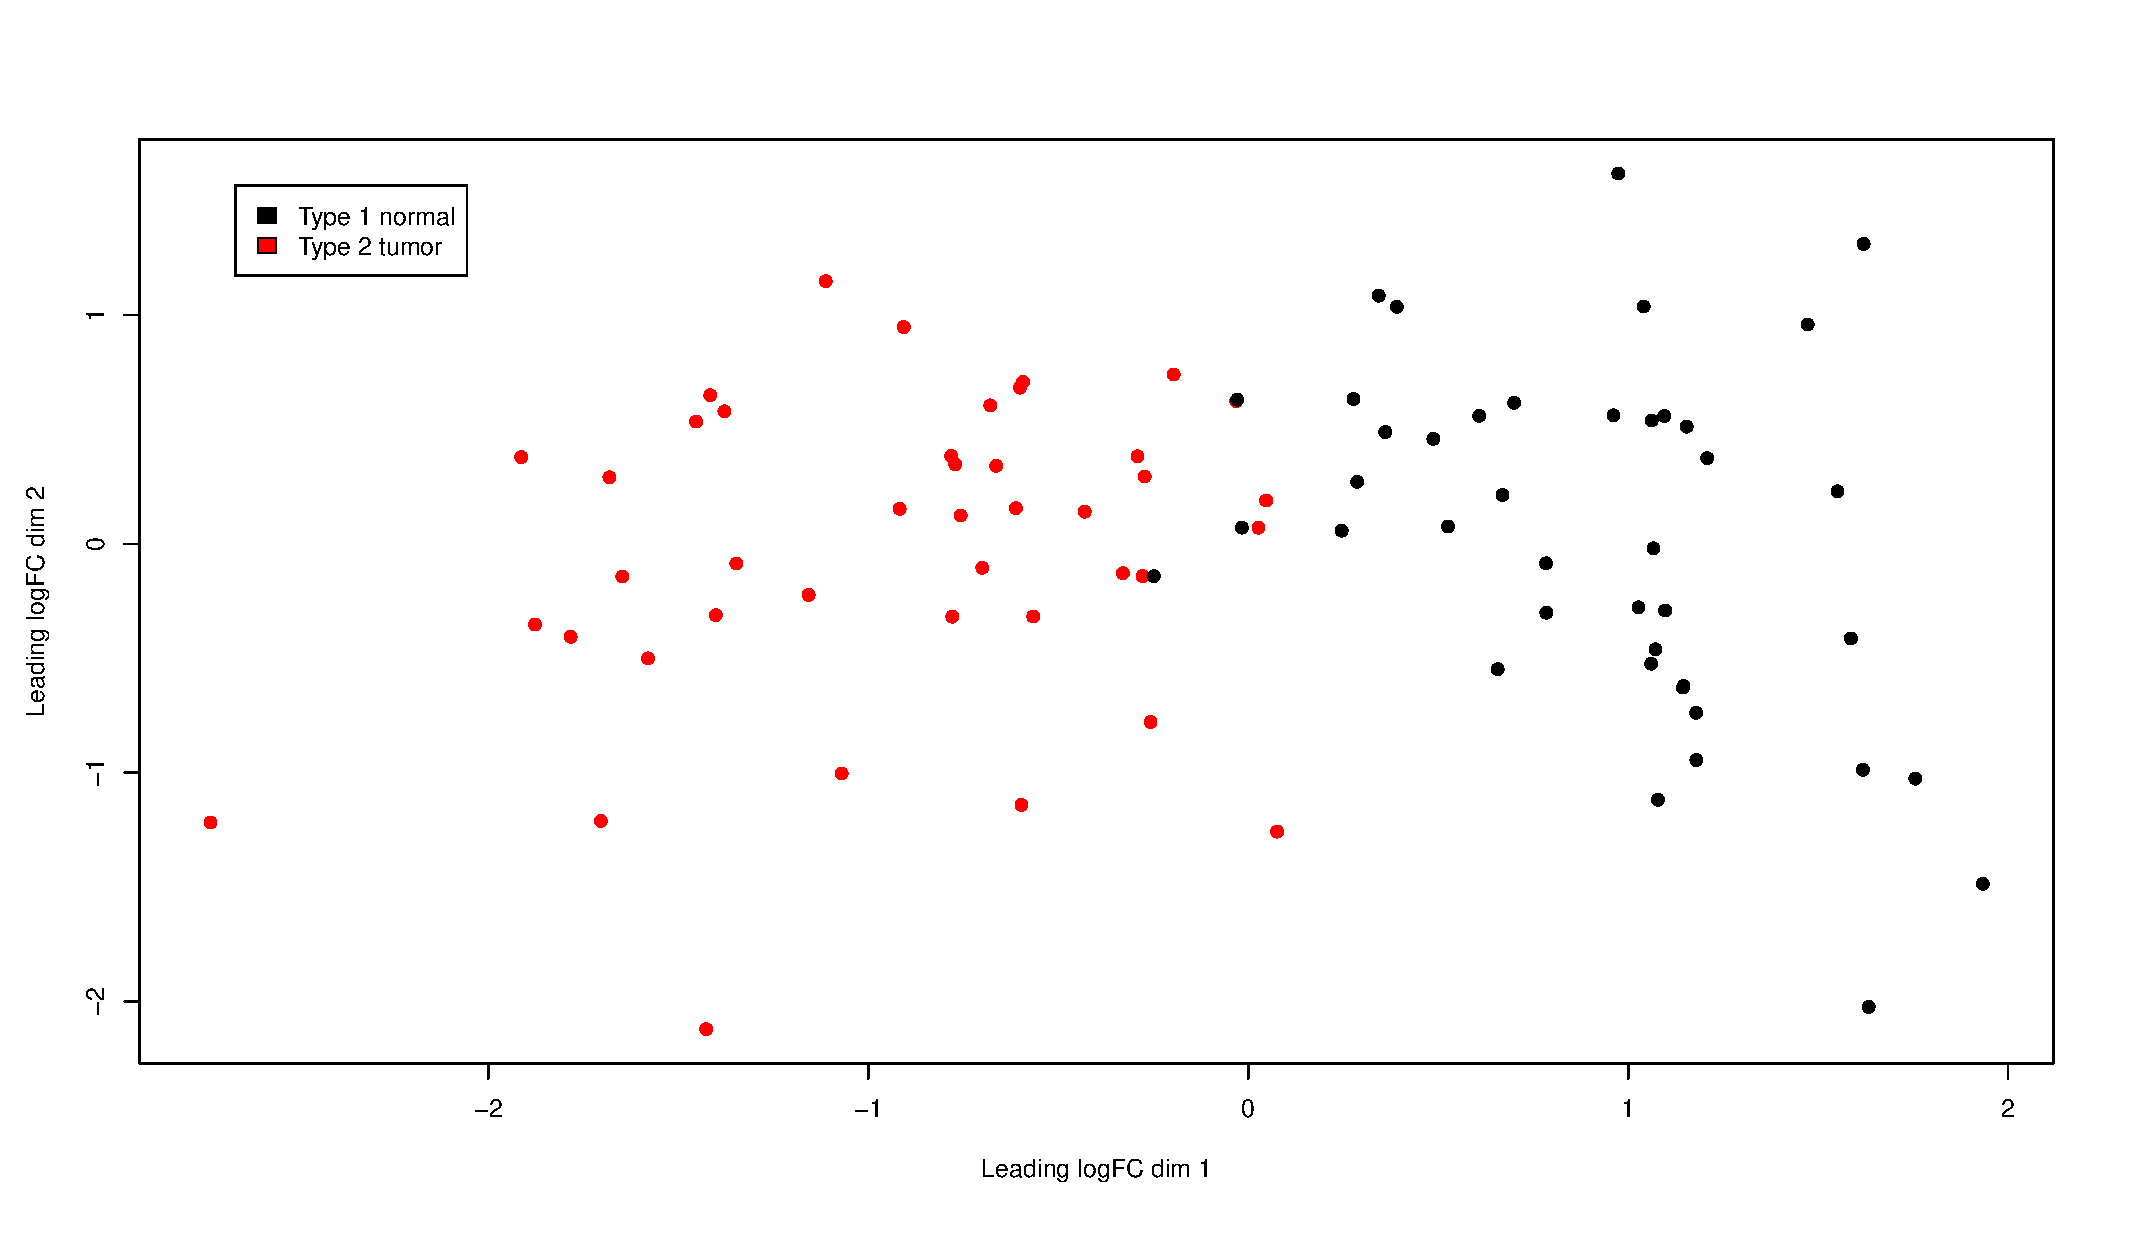
\includegraphics[width=0.8\textwidth,height=0.5\textheight,keepaspectratio]{mds4-1.eps}

\end{frame}

\begin{frame}{Methods}{Clustering}
	\centering
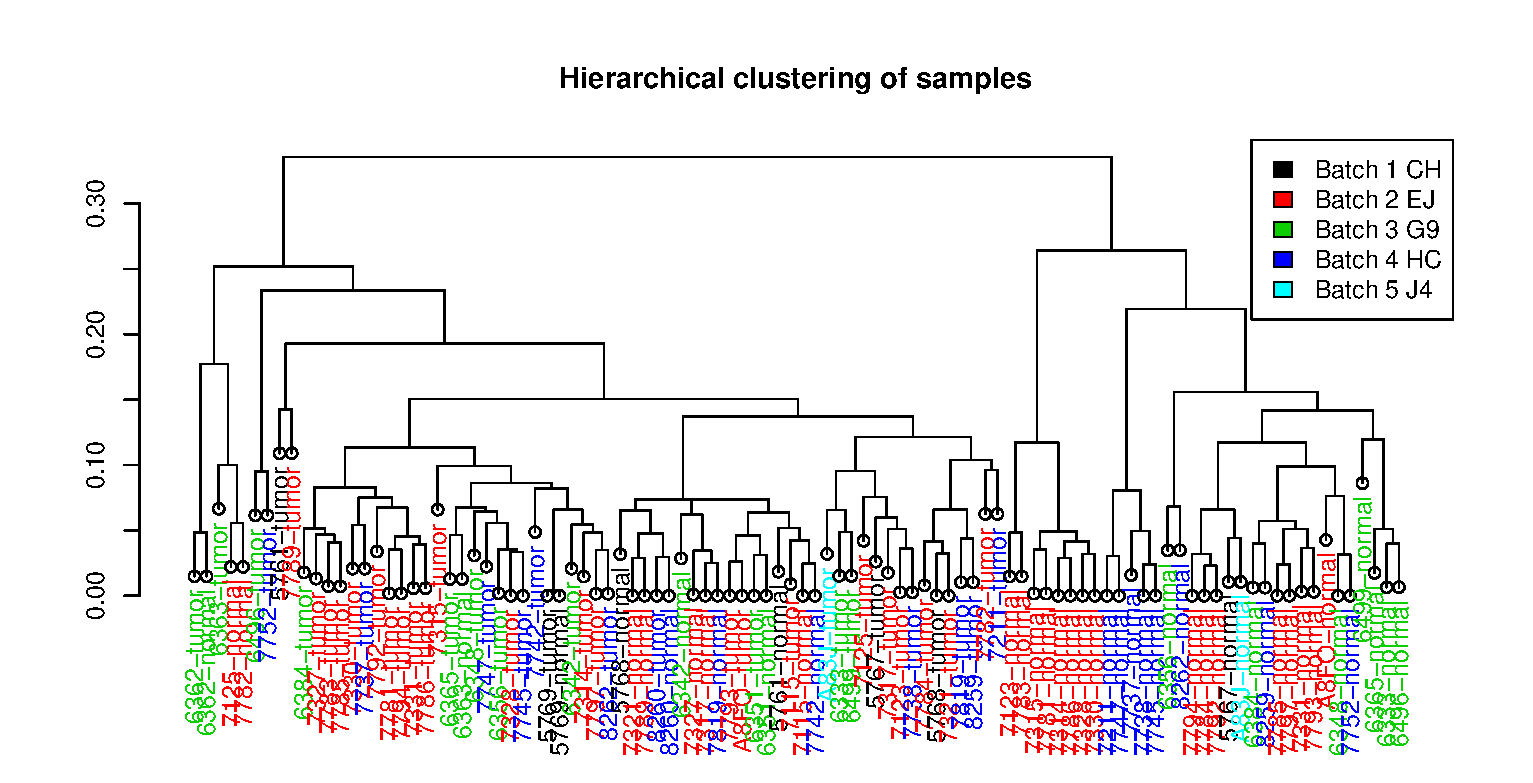
\includegraphics[width=.9\textwidth]{dendogram-1.eps}

\end{frame}

\begin{frame}{Methods}{HeatMap}
	\centering
	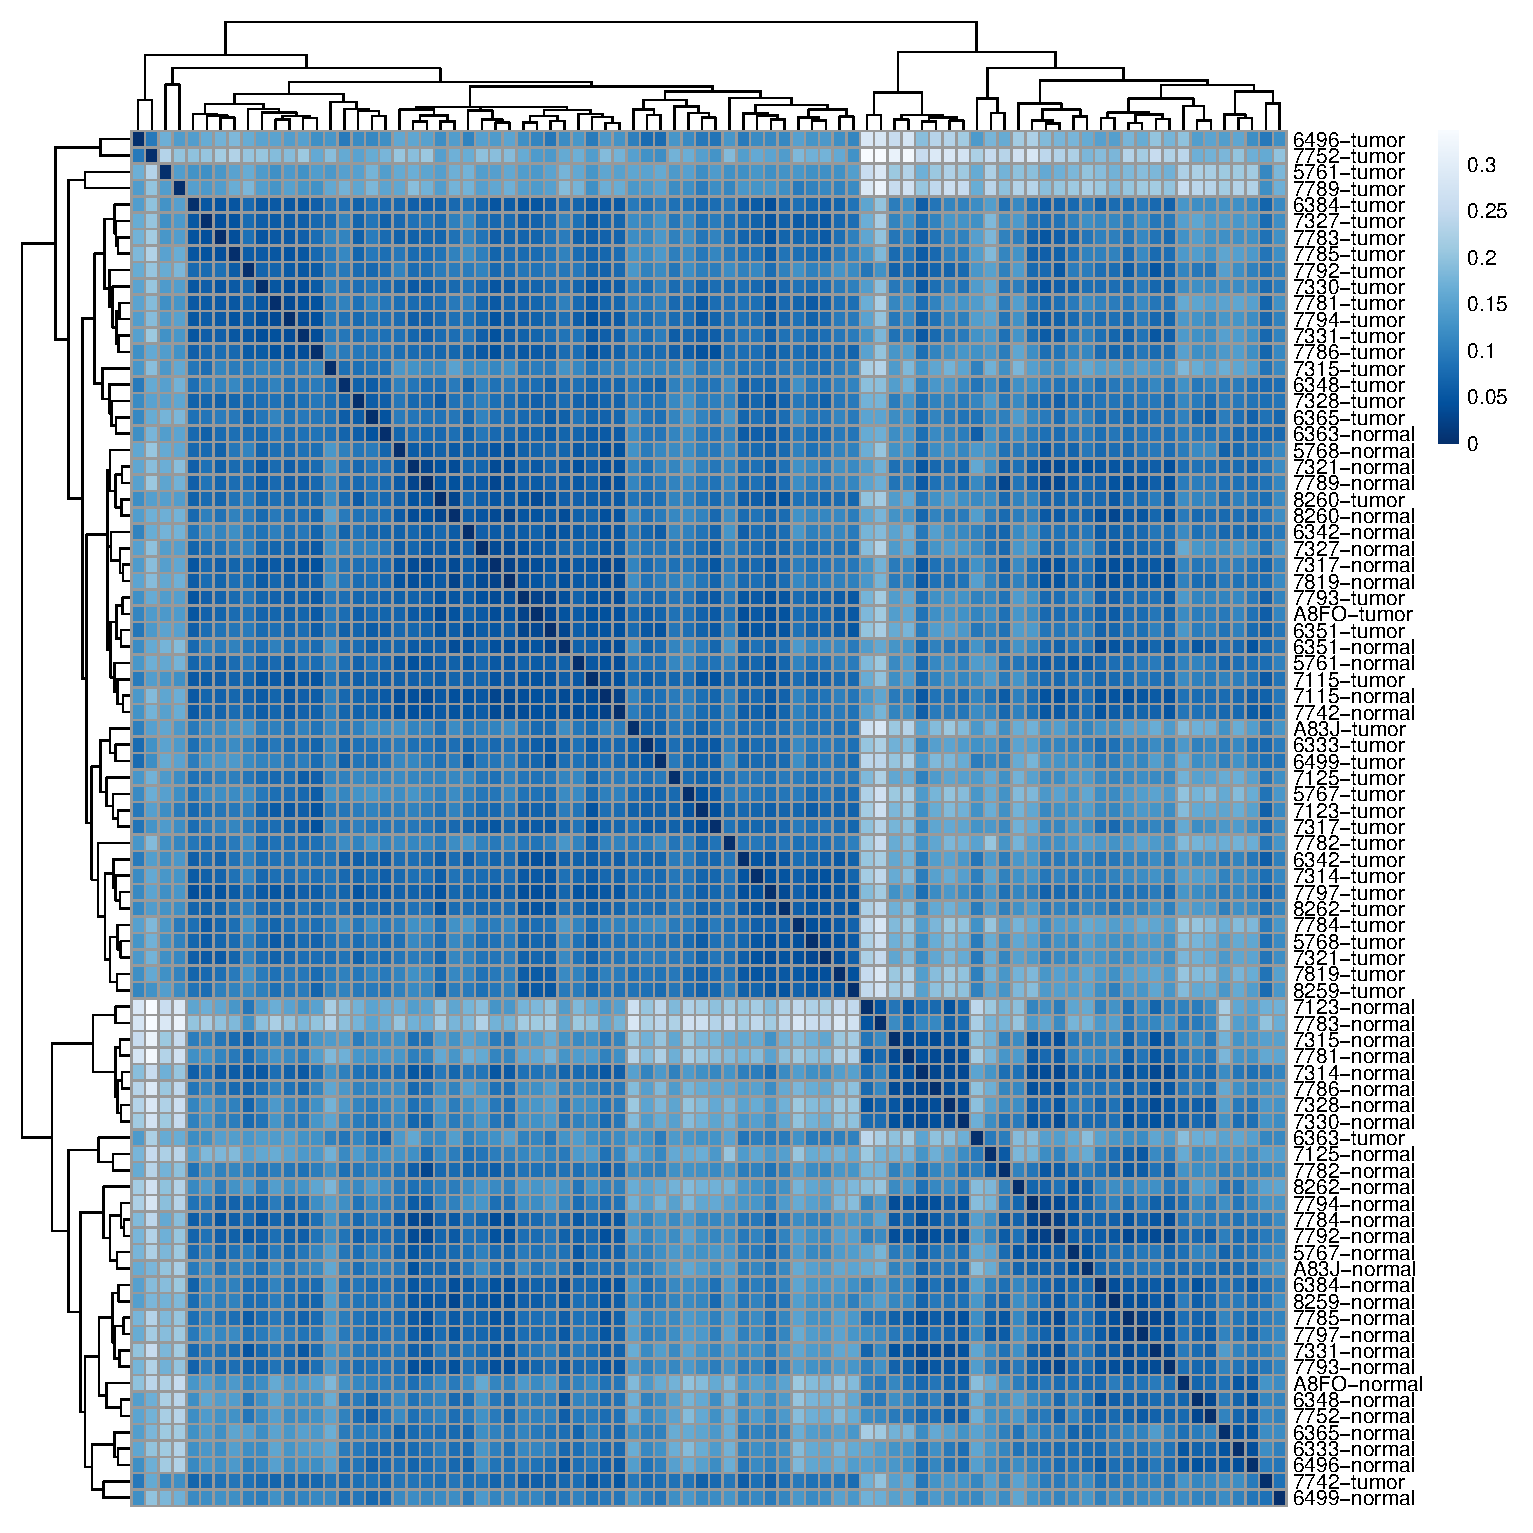
\includegraphics[width=0.70\textwidth,height=0.9\textheight,keepaspectratio]{Clustering.eps}

\end{frame}

\subsection{Statistical Analysis}

\begin{frame}{Methods}{Statistical Analysis}
	\begin{block}{SA: Differential Gene Expression}
		\begin{itemize}
			\item Voom correction (mean-variance correction).
			\item Surrogate Variables Analysis (SVA) was used \cite{leek2007capturing} \cite{svamanual}. Multiple Linear Regression (MLR)  and MA plots were used to analyse the data \cite{limma}.
			\item FDR = 0.001.
		\end{itemize}
	\end{block}
	\begin{block}{SA: Functional Enrichment}
		\begin{itemize}
			\item Gene Ontology sets were used for FE.
			\item GOstats package \cite{GOstats} was used.
		\end{itemize}
	\end{block}
	\begin{block}{SA: Gene Set Expression Analysis}
		\begin{itemize}
			\item Gene Set Enrichment Analysis (GSEA) \cite{GSEABase}.
			\item Gene Set Variation Analysis \cite{GSVA} \& \cite{GSVAdata}.
			\item KEGG \cite{kanehisa2016kegg}, Reactome \cite{fabregat2016reactome}, Biocarta \cite{nishimura2001biocarta} \& Prostat Cancer Gene Set.
		\end{itemize}
	\end{block}	
\end{frame}


\section{Results}


\subsection{DE genes}

\begin{frame}{Differential Gene Expression}{Volcano Plot}

   \begin{figure}
        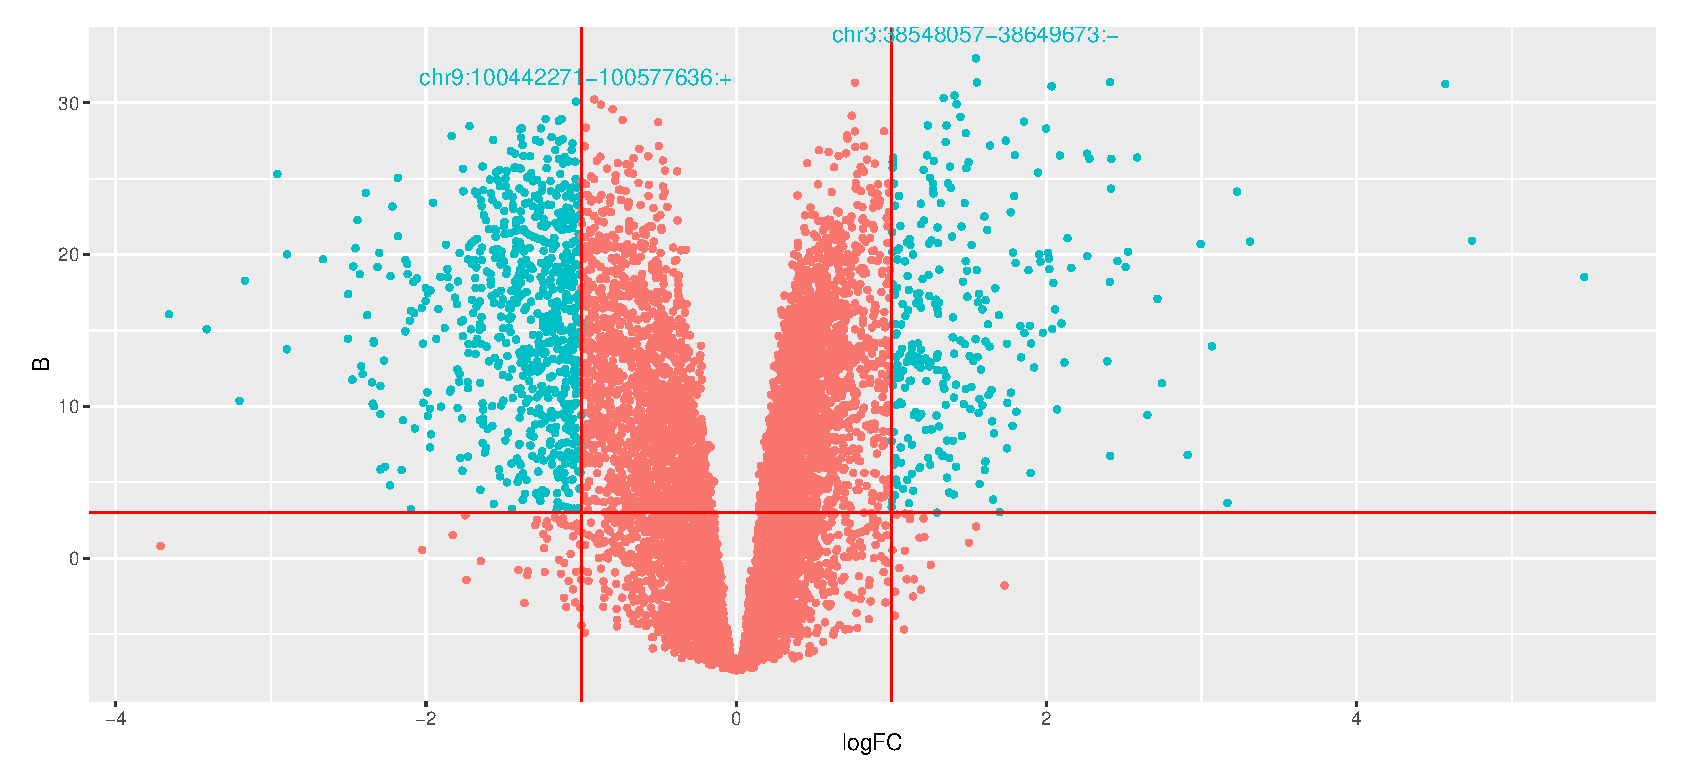
\includegraphics[width=1\textwidth]{Volcano.eps}
    \end{figure}

\end{frame}

\begin{frame}{Differential Gene Expression}{MA plots}

   \begin{figure}
        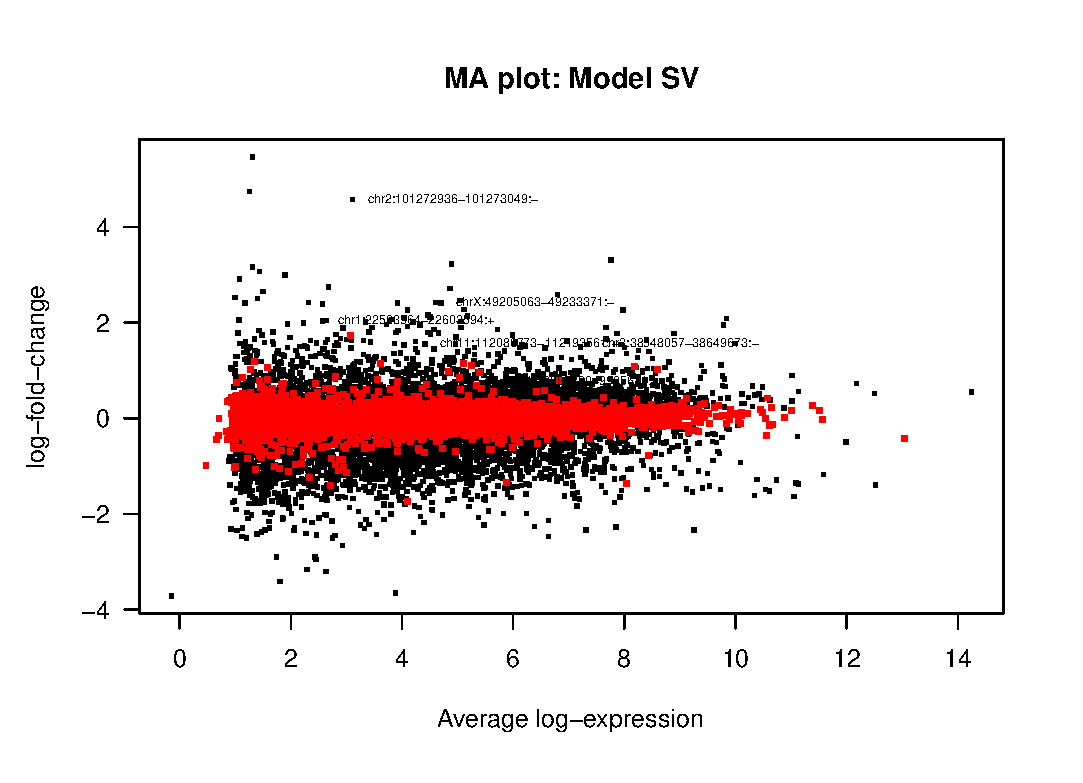
\includegraphics[width=0.8\textwidth,height=0.8\textheight,keepaspectratio]{MAplot.eps}
    \end{figure}

\end{frame}


\begin{frame}{Differential Gene Expression}{Top DE gene}

   \begin{figure}
        \includegraphics[width=0.8\textwidth,height=0.8\textheight,keepaspectratio]{SCN5A}
    \end{figure}

\end{frame}

\begin{frame}{Differential Gene Expression}{Top DE genes}
The Top5 Selected Gene through significance level: \cite{proteinatlas,uhlen2015tissue}
\begin{itemize}
	\item  EPHA8 - ephrin receptor, a neuronal factor.
    \item SNORD89 - small nucleolar RNA.
    \item SCN5A - sodium channel voltage gated V Type.
    \item AP002884.2  - putative gene 
    \item CACNA1F which is a calcium channel voltage dependant L type.
\end{itemize}
\pause
\begin{block}{Neuronal Connection}
Several DE genes present a connection with neuronal processes like EPHA8, SCN5A \& CACNA1F
\end{block}
\pause
\begin{block}{Mapping Error}
The AP002884.2 transcript compromises 2 genes SDHD and BCO2 related with the succinate dehydrogenase with vitamin A biosynthesis.\cite{kent2002human}
\end{block}
\end{frame}

\subsection{Functional Enrichment}
\begin{frame}{Functional Enrichment}{Selected GO terms}
\adjustbox{max width=\textwidth}{

\begin{tabular}{|c|r|r|r|r|r|p{2cm}|p{6cm}|}
 \hline
GOBPID & Pvalue & OddsRatio & ExpCount & Count & Size & Term & Genes \\ 
\hline
GO:0048710 & 0.00 & 11.20 & 7.53 &  13 &  14 & regulation of astrocyte differentiation & DAB1, EPHA4, F2, FGFR3, ATF5, PRPF19, BIN1, HES1, IL1B, NTRK3, SERPINE2, CNTN2, NR2E1 \\ 
GO:0033189 & 0.01 & 9.47 & 6.45 &  11 &  12 & response to vitamin A & DNMT3A, DNMT3B, GATA4, ARG1, LTC4S, RARA, RXRA, TSHB, TYMS, CAT, ALDH1A2 \\ 
 GO:0032309 & 0.01 & 6.03 & 8.60 &  14 &  16 & icosanoid secretion & ABCC4, ACE, DRD3, AGTR2, ACSL4, ANXA1, IL1B, NTSR1, OXT, P2RX7, BDKRB2, SYK, CYP4F2, TNFSF11 \\ 
GO:1901571 & 0.01 & 4.31 & 9.68 &  15 &  18 & fatty acid derivative transport & ABCC4, ACE, DRD3, AGTR2, ACSL4, ANXA1, IL1B, NTSR1, OXT, P2RX7, BDKRB2, SLCO2A1, SYK, CYP4F2, TNFSF11 \\ 
GO:0043966 & 0.01 & 3.45 & 13.45 &  20 &  25 & histone H3 acetylation & TRIM16, TAF6L, WDR5, CHEK1, KAT7, SGF29, DR1, BRD4, KAT6B, WBP2, SIN3A, BRPF3, PER1, PIH1D1, CSRP2BP, BRCA2, TAF10, BRPF1, KAT2B, SUPT7L \\ 
   \hline
\end{tabular}

}
\end{frame}

\subsection{Gene Set Expression Analysis}


\begin{frame}{Gene Set Expression Analysis}{ Enrichment approach (GSEA)}
\adjustbox{max width=\textwidth}{
\begin{tabular}{|l|c|c|p{6.3cm}|}
 \hline
Gene Set & Relative tumor expression &  Z-value & Genes \\
  \hline
REACTOME DEADENYLATION OF MRNA & Over-Expressed  & 19.19 & EIF4A1, EIF4A2, EIF4B, EIF4E, EIF4G1, CNOT2, CNOT4, RQCD1, CNOT8, PAN2, CNOT1, CNOT10, PABPC1, CNOT7, CNOT6, TNKS1BP1, CNOT6L, PAN3 \\
REACTOME SMOOTH MUSCLE CONTRACTION & Under-Expressed & 18.70 & ACTA2, ACTG2, CALM1, CALM3, ITGA1, ITGB5, PXN, TPM2, VCL, SORBS1 \\
REACTOME BOTULINUM NEUROTOXICITY & Over-Expressed &  17.62 & SNAP25, SYT1, STX16, STX11, STX10, STX6, STX12, STX1B \\
REACTOME ENDOGENOUS STEROLS & Under-Expressed & 17.54 & CYP8B1, CYP11B1, CYP51A1, CYP46A1, CYP39A1 \\
\hline
\end{tabular}
}
\end{frame}

\begin{frame}{Gene Set Expression Analysis}{ Enrichment approach (GSEA)}
\centering 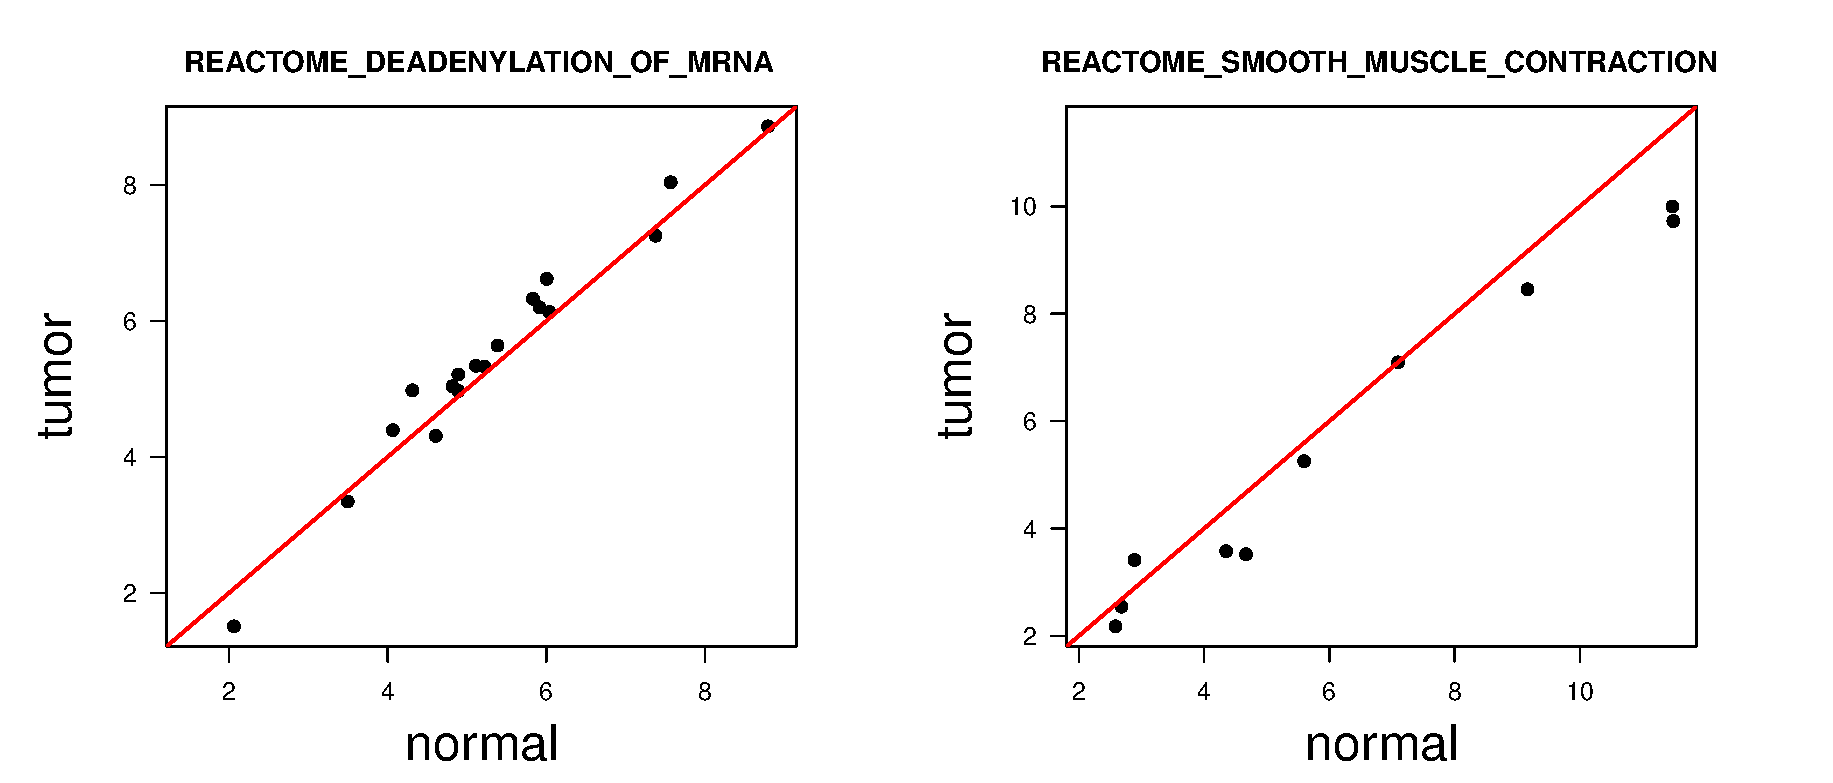
\includegraphics[width=0.8\textwidth,height=0.4\textheight,keepaspectratio]{genesets1.eps} \\
        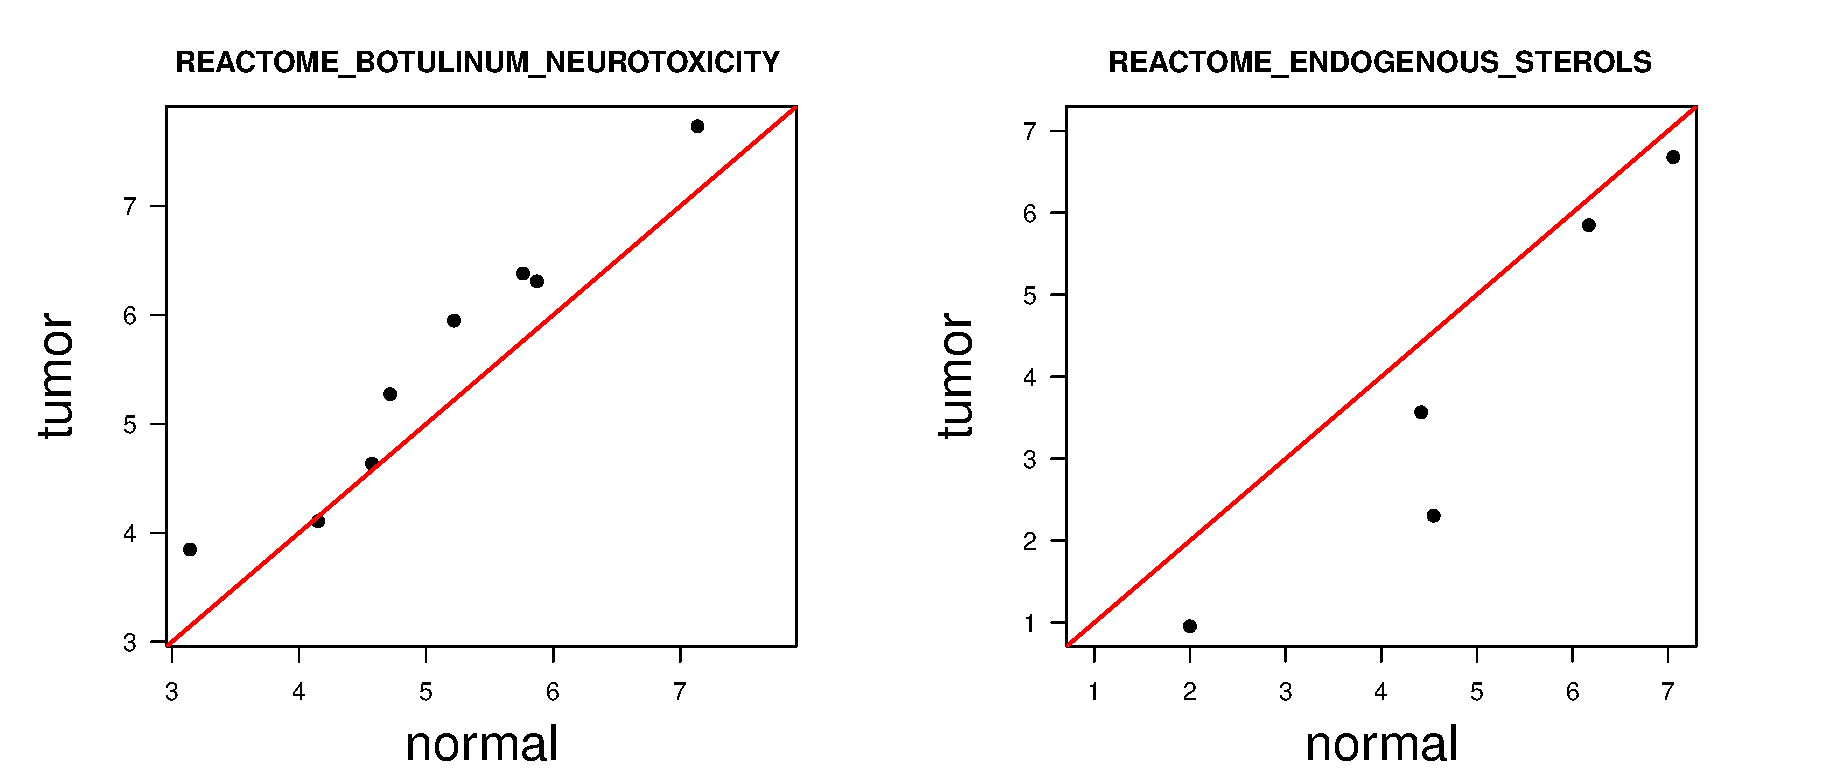
\includegraphics[width=0.8\textwidth,height=0.4\textheight,keepaspectratio]{genesets2.eps}
\end{frame}

\begin{frame}{Gene Set Expression Analysis}{ Variation  approach (GSVA)}
   \centering
        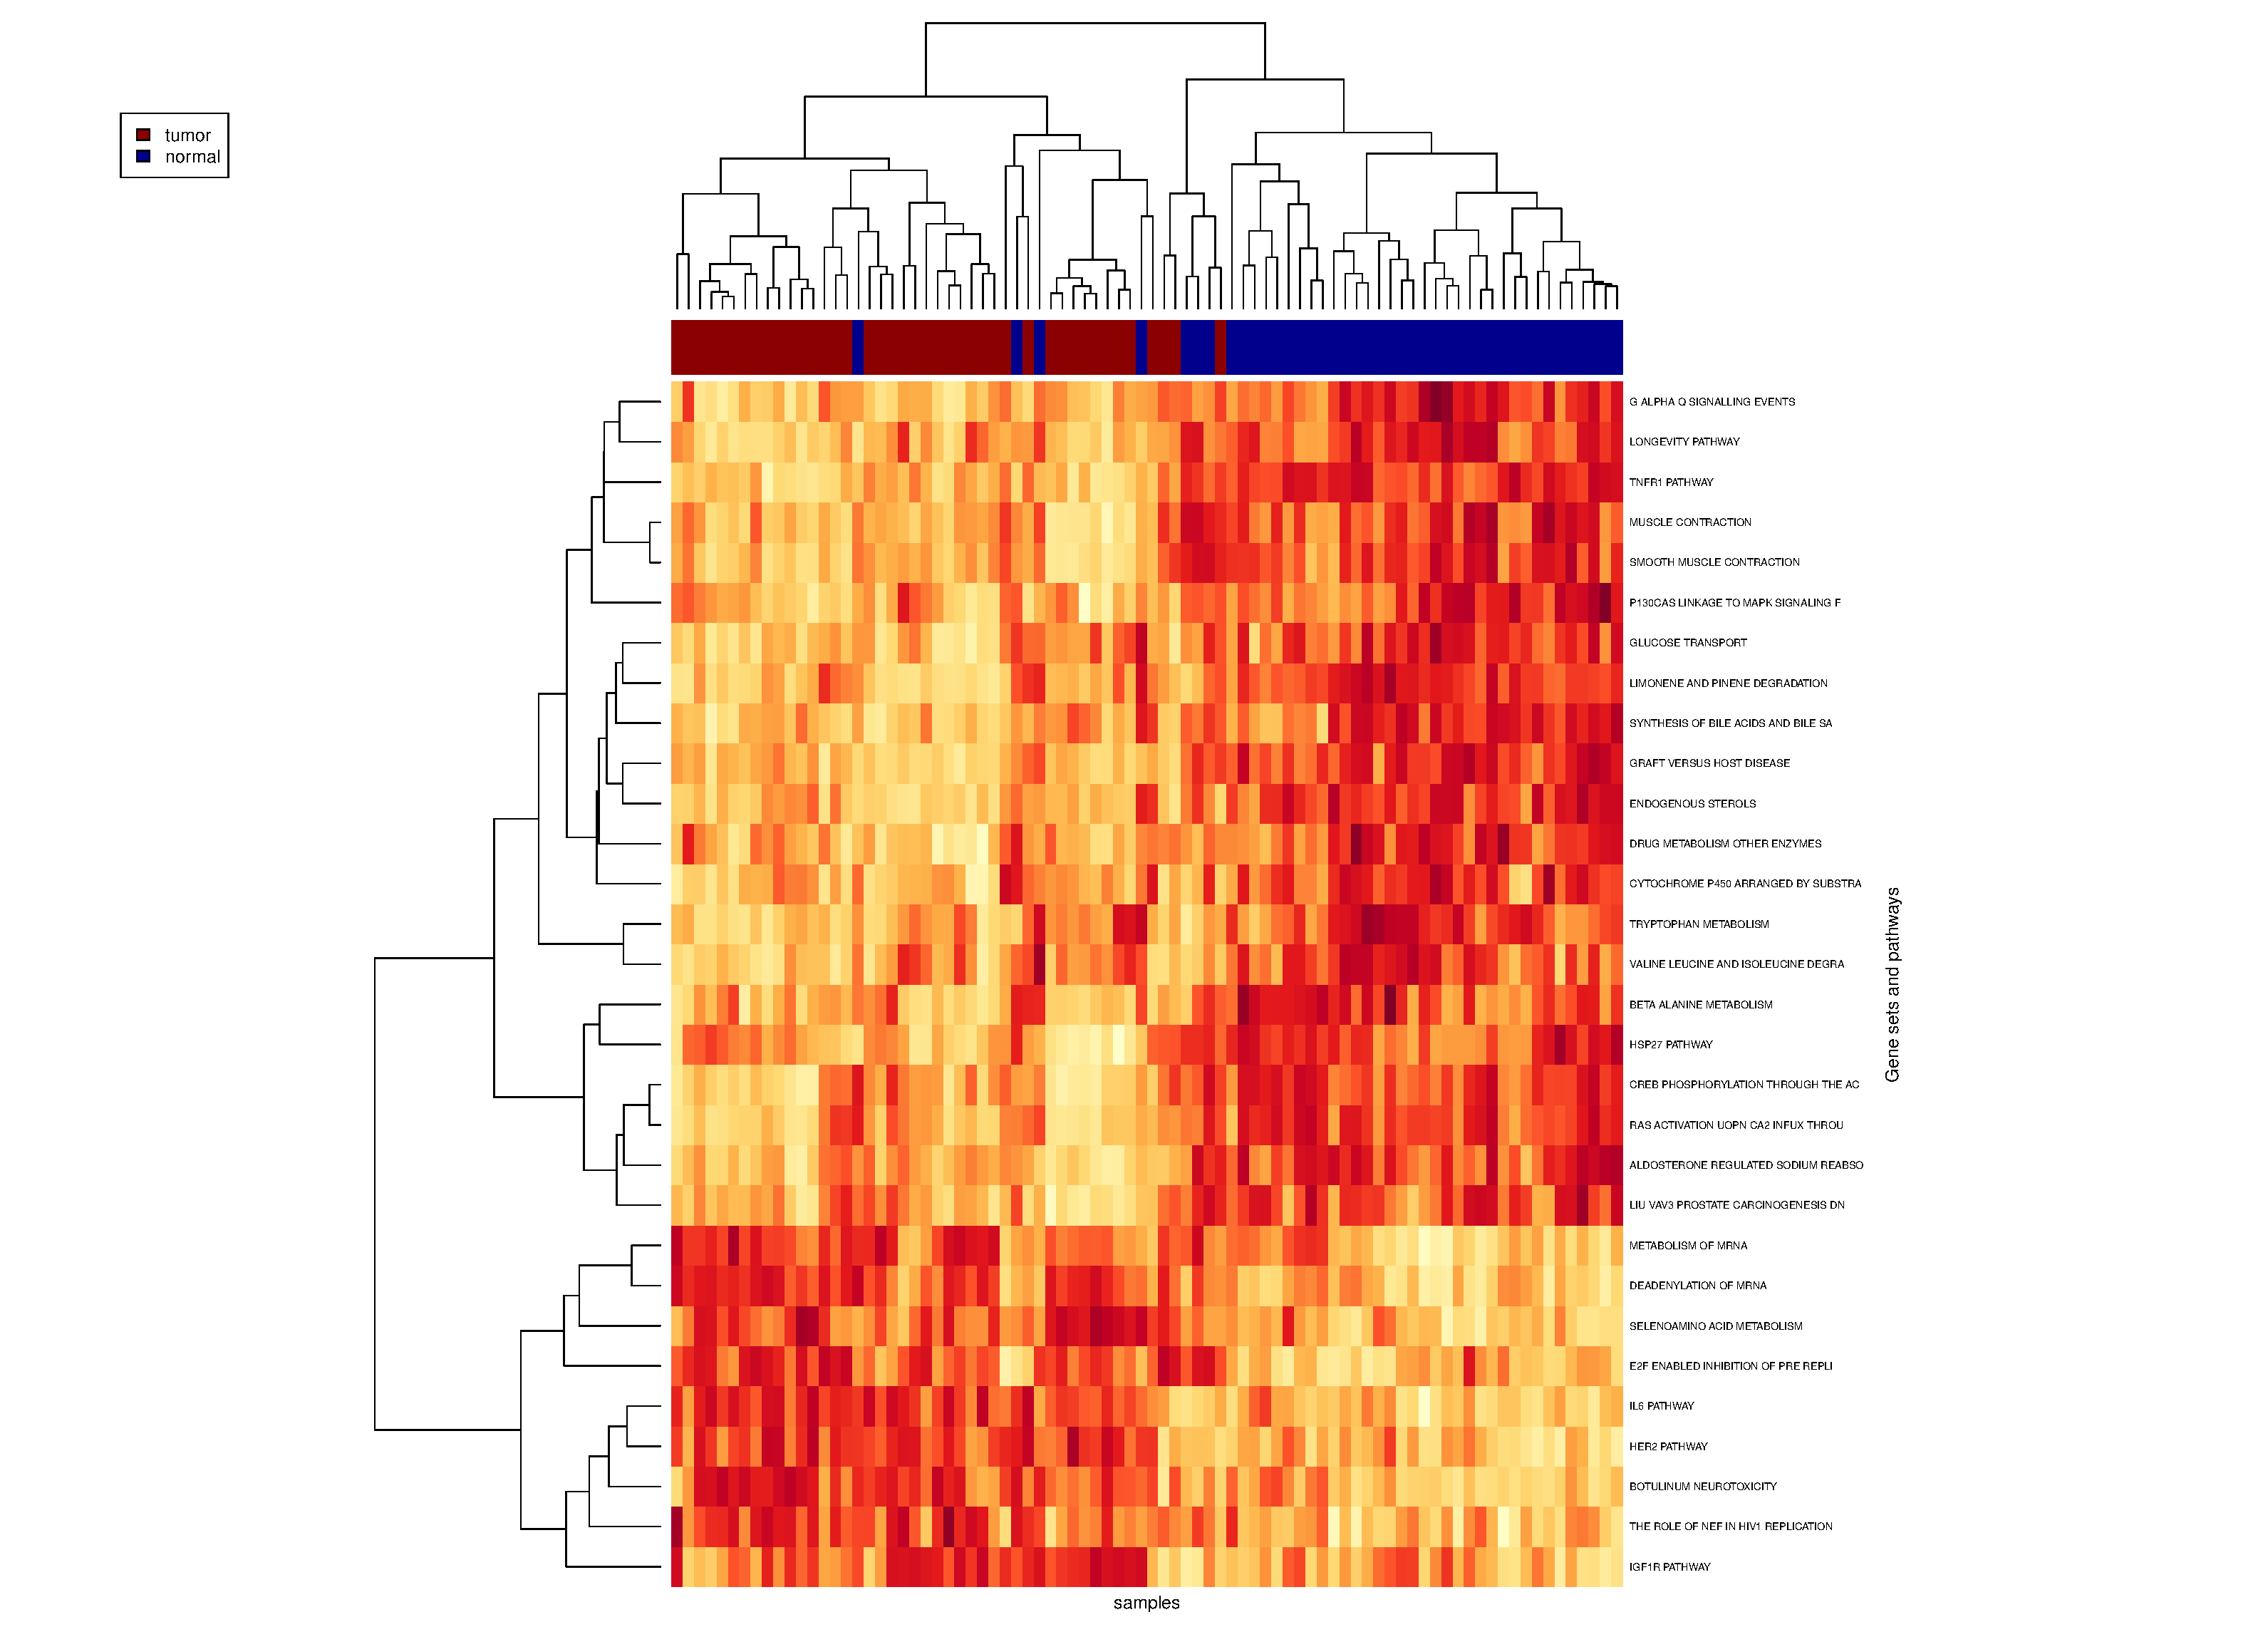
\includegraphics[width=1\textwidth,height=0.8\textheight,keepaspectratio]{ClusteringGSVA.eps}

\end{frame}


\begin{frame}{Gene Set Expression Analysis}{ Comparison}
\centering
        \includegraphics[width=.7\textwidth,height=0.8\textheight,keepaspectratio]{venn}
\end{frame}




\section{Conclusions}

\begin{frame}{Summary}
  \begin{itemize}
  \item
    The \alert{first main message} of your talk in one or two lines.
  \item
    The \alert{second main message} of your talk in one or two lines.
  \item
    Perhaps a \alert{third message}, but not more than that.
  \end{itemize}
  
  \begin{itemize}
  \item
    Outlook
    \begin{itemize}
    \item
      Something you haven't solved. 
    \item
      Something else you haven't solved.
    \end{itemize}
  \end{itemize}
\end{frame}



% All of the following is optional and typically not needed. 
\appendix
\section<presentation>*{\appendixname}
\subsection<presentation>*{For Further Reading}


\begin{frame}[allowframebreaks]%in case more than 1 slide needed
\frametitle<presentation>{References}
    {\footnotesize
    \bibliographystyle{unsrt}
    \bibliography{prac-bibliography}
    }
\end{frame}


\end{document}


